\subsection{Normalized Device Coordinates (NDC)}

In Normalized Device Coordinates, $x$, $y$ and $z$ $\in [-1,1]$. This is the default coordinate system in OpenGL. The following image shows the NDC space.

\begin{center}
    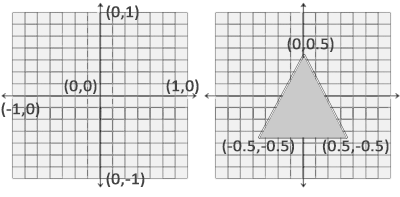
\includegraphics[scale = 3]{pics/ndc.png}
\end{center}

\subsection{Graphics Pipeline}

The order with which OpenGL proccesses vertex data:

\begin{center}
    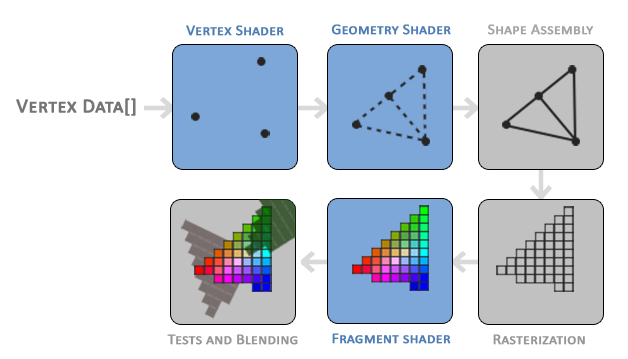
\includegraphics[scale = 2]{pics/pipeline.png}
\end{center}

\subsection{Vertex Buffer Data}

Vertex attributes are stored in the following order:

\begin{center}
    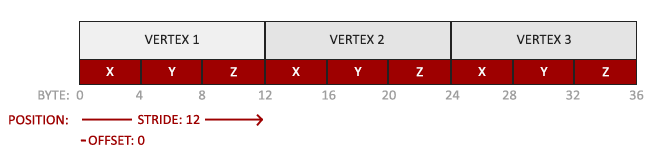
\includegraphics[scale = 0.5]{pics/vertex_attribute_pointer.png}
\end{center}

Vertices are stored in the Vertex Buffer Object (VBO).

\subsection{VBO, VAO, EBO}

\begin{itemize}
    \item \textbf{VBO} stores vertex data (e.g., positions, normals, colors) in GPU memory. \red{It allows efficient transfer of vertex data to the GPU, enabling faster rendering. You bind a VBO and then specify the vertex data using functions like glBufferData.}
    \item \textbf{VAO} stores the configuration of vertex attributes and their associated buffers. \red{It simplifies the process of switching between different vertex data configurations. When you bind a VAO, it automatically sets up the vertex attribute pointers and buffer bindings.}
    \item \textbf{EBO} stores indices that define the order in which vertices should be drawn. \red{It helps in reducing the amount of vertex data needed by reusing vertices. You bind an EBO and specify the indices using functions like glBufferData.}
\end{itemize}